\section*{Descripción Textual del Proceso Interno: Agregar Cuerpos}

\subsubsection{Objetivo del Proceso}
Incorporar un cuerpo celeste con propiedades físicas $(m, \mathbf{x}, \mathbf{v})$ a una simulación REBOUND existente, permitiendo:
\begin{itemize}
    \item Configuración de sistemas de 2 cuerpos
    \item Cálculo posterior de estabilidad dinámica (LE)
    \item Integración en el ciclo de optimización
\end{itemize}

\subsubsection{Entradas Principales}
\begin{itemize}
    \item \textbf{sim}: Referencia a objeto \texttt{Simulation} de REBOUND
    \item \textbf{body\_params}: Estructura con:
    \begin{itemize}
        \item $m \in \mathbb{R}^+$ (masa)
        \item $\mathbf{x} = [x, y, z]$ (posición inicial)
        \item $\mathbf{v} = [v_x, v_y, v_z]$ (velocidad inicial)
    \end{itemize}
\end{itemize}

\subsubsection{Sub-pasos Secuenciales}
Este apartado es proporcionado para profundizar y describir de forma textual cada paso contenido dentro del diagrama del proceso descrito en la figura~\ref{fig:process_diagram05}
\subsubsection*{1. Recibir Parámetros}
\begin{itemize}
    \item Capturar \texttt{sim} y \texttt{body\_params}
\end{itemize}

\subsubsection*{2. Desempaquetar Parámetros}
\begin{itemize}
    \item Extraer: $m, x, y, z, v_x, v_y, v_z$
\end{itemize}

\subsubsection*{3. Validación Opcional}
\begin{itemize}
    \item Chequear:
    \begin{itemize}
        \item $\forall v \in \{m, x, y, z, v_x, v_y, v_z\}: v \neq \text{NaN}, \infty$
        \item $m > 0$
    \end{itemize}
\end{itemize}

\subsubsection*{4. Invocar API REBOUND}
\begin{verbatim}
sim.add(m=m, x=x, y=y, z=z,
        vx=vx, vy=vy, vz=vz)
\end{verbatim}

\subsubsection*{5. Procesamiento Interno REBOUND}
\begin{itemize}
    \item Asignar memoria para nueva partícula
    \item Actualizar contador: $n_{\text{partículas}} \leftarrow n_{\text{partículas}} + 1$
    \item Recalcular propiedades del sistema (opcional)
\end{itemize}

\subsubsection*{6. Verificación de Estado (Opcional)}
\begin{itemize}
    \item Confirmar $n_{\text{partículas}} = n_{\text{prev}} + 1$
\end{itemize}

\subsubsection{Lógica Interna y Decisiones}
\begin{itemize}
    \item \textbf{Flujo lineal}: Sin bifurcaciones principales
    \item \textbf{Validaciones}:
    \begin{itemize}
        \item Opcionales, dependientes de implementación
        \item Manejo de errores delegado a REBOUND
    \end{itemize}
\end{itemize}

\subsubsection{Manejo de Datos Específico}
\begin{itemize}
    \item \textbf{Entradas}:
    \begin{itemize}
        \item Referencia a simulación existente
        \item Parámetros físicos estructurados
    \end{itemize}
    \item \textbf{Intermedios}:
    \begin{itemize}
        \item Estructura interna de partícula en REBOUND
    \end{itemize}
    \item \textbf{Salida}:
    \begin{itemize}
        \item Simulación modificada in-place
    \end{itemize}
\end{itemize}

\subsubsection{Salidas Principales}
\begin{itemize}
    \item \texttt{sim} actualizado con nuevo cuerpo
    \begin{itemize}
        \item Listo para integración numérica
        \item Configuración adicional posible
    \end{itemize}
\end{itemize}

\subsubsection{Interacciones Internas}
\begin{itemize}
    \item \textbf{Con API REBOUND}:
    \begin{itemize}
        \item Método \texttt{add~()} para gestión de partículas
        \item Administración interna de memoria
    \end{itemize}
    \item \textbf{Con subsistema físico}:
    \begin{itemize}
        \item Actualización de propiedades del sistema
    \end{itemize}
\end{itemize}

\subsubsection{Diagrama del Proceso}
\begin{figure}[H]
    \centering
    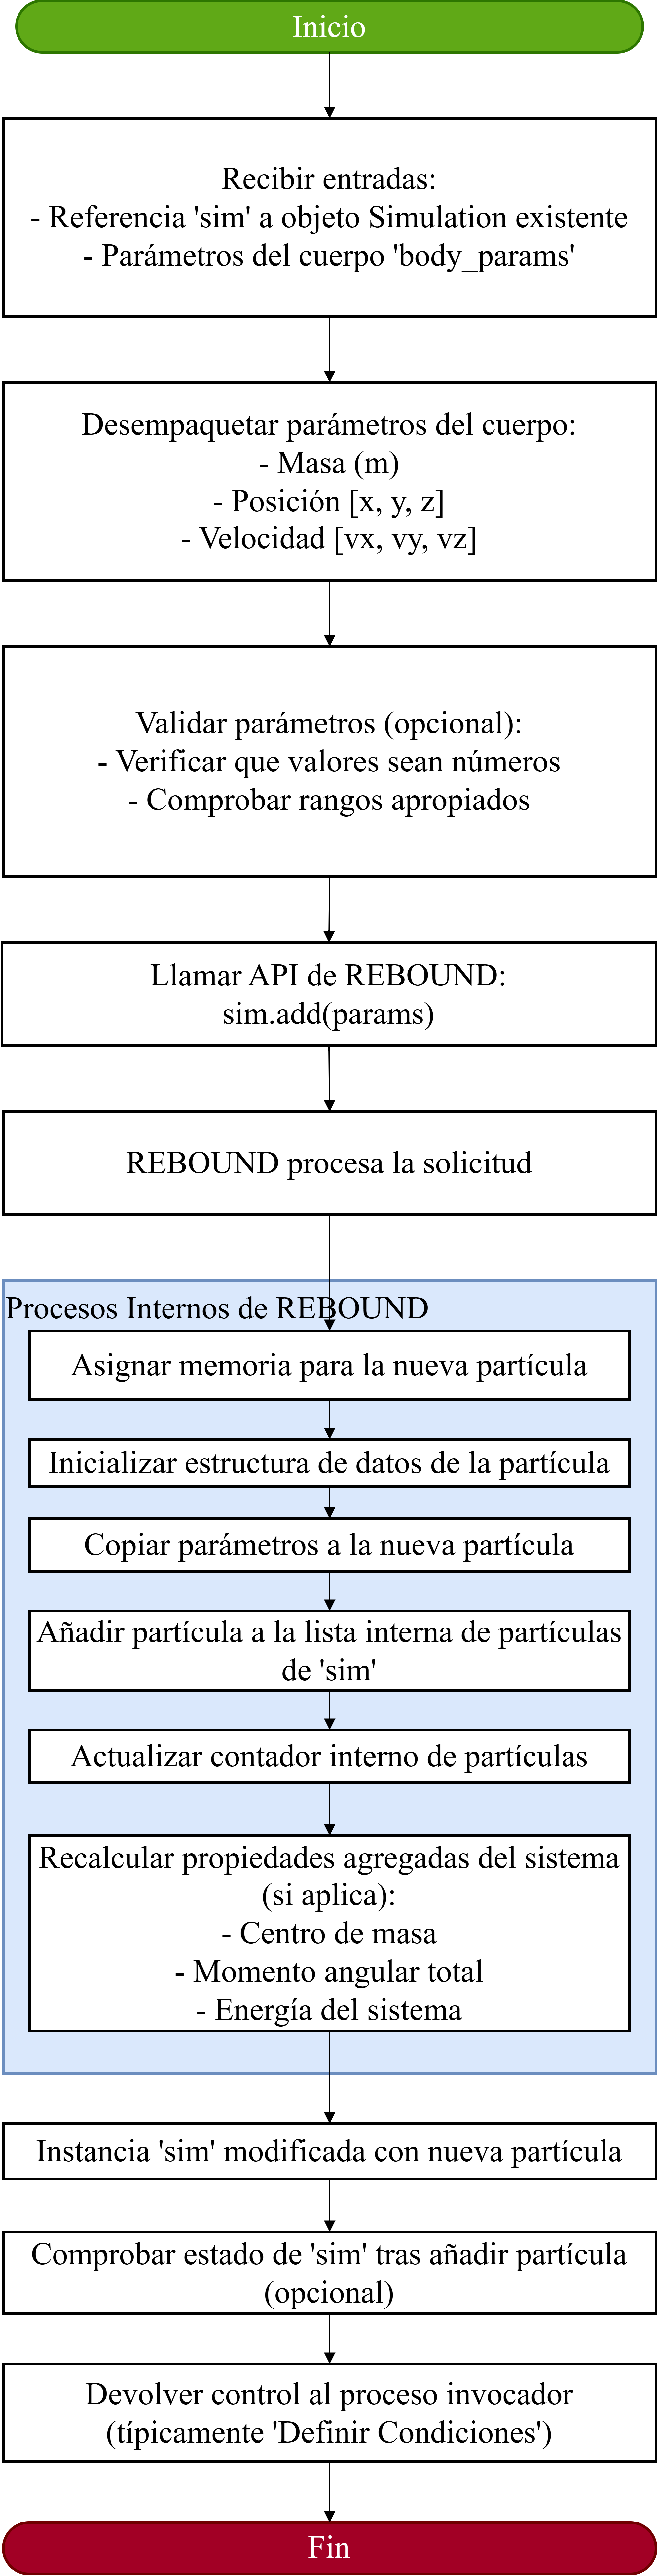
\includegraphics[width=\textwidth]{img/Analisis/DiagramaProcesos/DiagramaProceso05AgregarCuerpos.png}
    \caption{Diagrama de Proceso Interno 05: Agregar Cuerpos}%
    \label{fig:process_diagram05}
\end{figure}